This chapter presents a number of benchmarks used to compare the OpenQuake-engine
hazard results against solutions provided by alternative software. The focus is on simple test cases which involve a single source typology at a time and no epistemic uncertainties. The end goal is to investigate discrepancies in modeling the same source typolgy in different software. Classical PSHA results (i.e. hazard curves and maps) generated by the OpenQuake-engine are compared against solutions computed using the the suite of seismic hazard analysis computer programs developed by the United States Geological Survey - National Seismic Hazard Program (USGS-NSHMP).
% ..............................................................................
\section{Comparison against the USGS-NSHMP computer programs}
The USGS-NSHMP developed a number of Fortran-based computer programs used to implement the U.S. national seismic hazard model (\cite{petersen2008}). Source codes are available on the internet (http://earthquake.usgs.gov/hazards/products/conterminous/2008/software/) together with input files containing the seismic hazard model definition. Input files are available for the three main source typologies
defined in the U.S. national seismic hazard model: distributed seismicity, crustal faults and subduction faults.
The USGS-NSHMP seismic hazard software offers therefore an excellent opportunity to test the OpenQuake-engine algorithms for the different seismic source typologies.

\subsection{Benchmarks for distributed seismicity}
As a benchmark for the modeling of distributed seismicity we selected a gridded seismicity model developed for the State of California (Figure \ref{fig:cal_grid}). The model is associated with the USGS-NSHMP computer program for gridded seismicity \textit{hazgridXnga3.f}. 

The model defines spatially variable occurrence rates over a regular grid (0.1 by 0.1 degrees) obtained using a smoothed seismicity approach (\cite{frankel1995}). Occurrence rates are defined from minimum magnitude equal to 5. Maximum magnitude is equal to 7 in areas away from faults. Close to faults, the maximum magnitude is assumed equal to the minimum between 7 and the fault's maximum magnitude. Occurrence rates follow a double truncated Gutenberg-Richter magnitude frequency distribution with $b_{GR} = 0.8$. Rupture extension is modeled using the magnitude-length scaling relationship of \citet{wells1994} for the 'All Slip Types' case ($L=10^{-3.22+0.69 M}$). The rupture top edge is placed at 0 km depth for $M \ge 6.5$ and at 5 km depth for  $M < 6.5$.

We compared hazard curves on a set of 21 equally spaced locations defining a profile connecting San Francisco (-122.42W, 37.78N) to Los Angeles (-118.25E, 34.05N). We computed hazard curves (probabilities of exceedance in 50 years) for peak ground acceleration using the \citet{boore2008} GMPE. This GMPE requires as distance metrics the Joyner-Boore distance ($R_{JB}$). 

We first computed hazard curves under the assumption of \textit{point ruptures}. That is ruptures are treated as having no spatial extension. Under this assumption $R_{JB}$ converges to epicentral distance. Results of the comparison (as PGA values for different return periods along the profile) are given in Figure \ref{fig:cal_grid_map_point}. Comparison of hazard curves at a single site is also given in Figure \ref{fig:cal_grid_curve_point}. For most of the locations, results are in agreement. For few sites, larger discrepancies are observed that increase with increasing return periods.

A second test is performed but considering extended ruptures. For simplicity, ruptures are assumed vertical and aligned along a single strike direction ($0^{\circ}$). All ruptures are assumed to be strike-slip. In the OQ-engine calculation, the rupture extension is modeled by considering the \textit{magnitude-area} scaling relationship of \citet{wells1994} ($A = 10^{-3.42 + 0.90 M}$) and assuming an aspect ratio equal to 1. In the \textit{hazagridXnga3.f} rupture extension is modeled based on the \textit{magnitude-length} scaling relationship of \citet{wells1994} ($L = 10^{-3.22+0.69 M}$).

Results of the comparison are given in Figures \ref{fig:cal_grid_map_finite} and \ref{fig:cal_grid_curve_finite}. Discrepancies are much larger than under the \textit{point ruptures} approximations, at all return periods. This can be motivated by the fact that the two software adopt different modeling strategies. The OQ-engine uses a magnitude-area scaling relationship which implies that rupture length may be increased if, for given area and rupture aspect ratio, the resulting rupture width is larger than the seismogenic layer thickness. On the contrary, in the USGS-NSHMP approach, rupture extension is constrained by a magnitude-length scaling relationship. For the same rupture magnitude, the OQ-engine may predict shorter distances and thus provide higher hazard values. For a more detailed analysis on the differences between the OpenQuake-engine and the USGS-NSHMP approach in modeling distributed seismicity we refer to the work of \citet{monelli2014}.

\begin{figure}
\centering
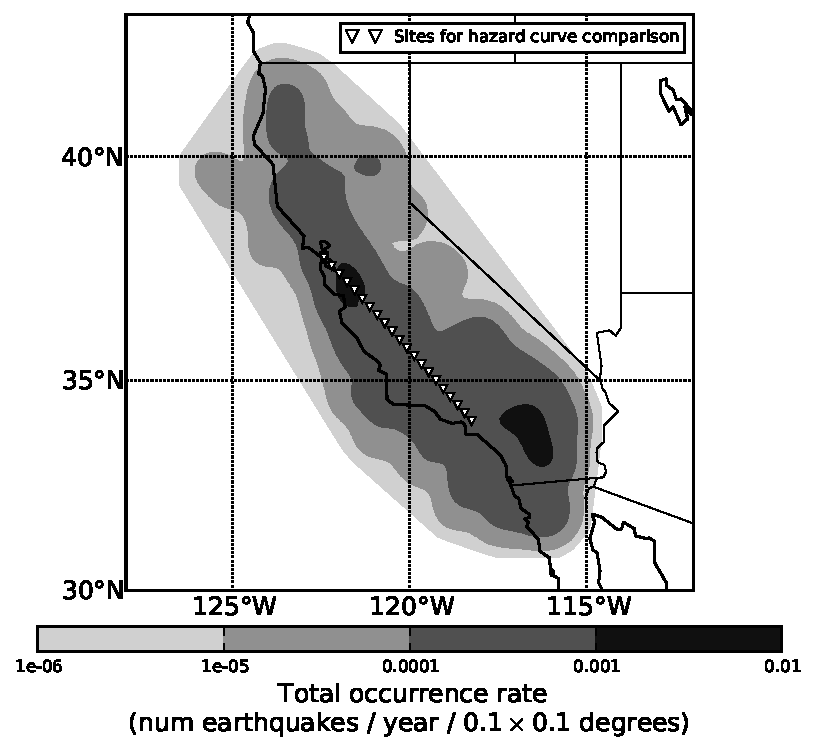
\includegraphics[width=10cm]{./qareport/pictures/CAmapC_21.pdf}
\caption{Gridded seismicity model used as benchmark for testing distributed seismicity in the OQ-engine. Hazard curves are compared for a set of 21 sites defining a profile connecting San Francisco to Los Angeles.}
\label{fig:cal_grid}
\end{figure}


\begin{figure}
\centering
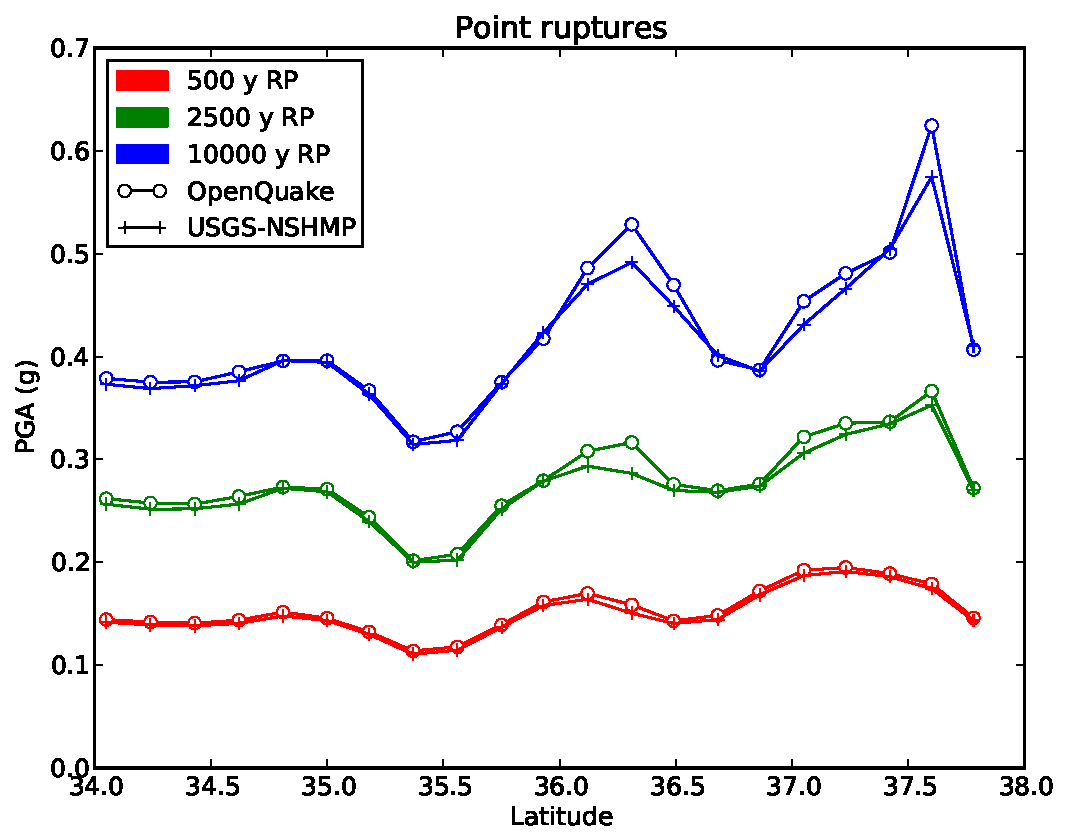
\includegraphics[width=10cm]{./qareport/pictures/gridded_seismicity_oq_nshmp_point.pdf}
\caption{Comparison of hazard map values for different return periods (RP) along the profile assuming \textit{point ruptures}}
\label{fig:cal_grid_map_point}
\end{figure}

\begin{figure}
\centering
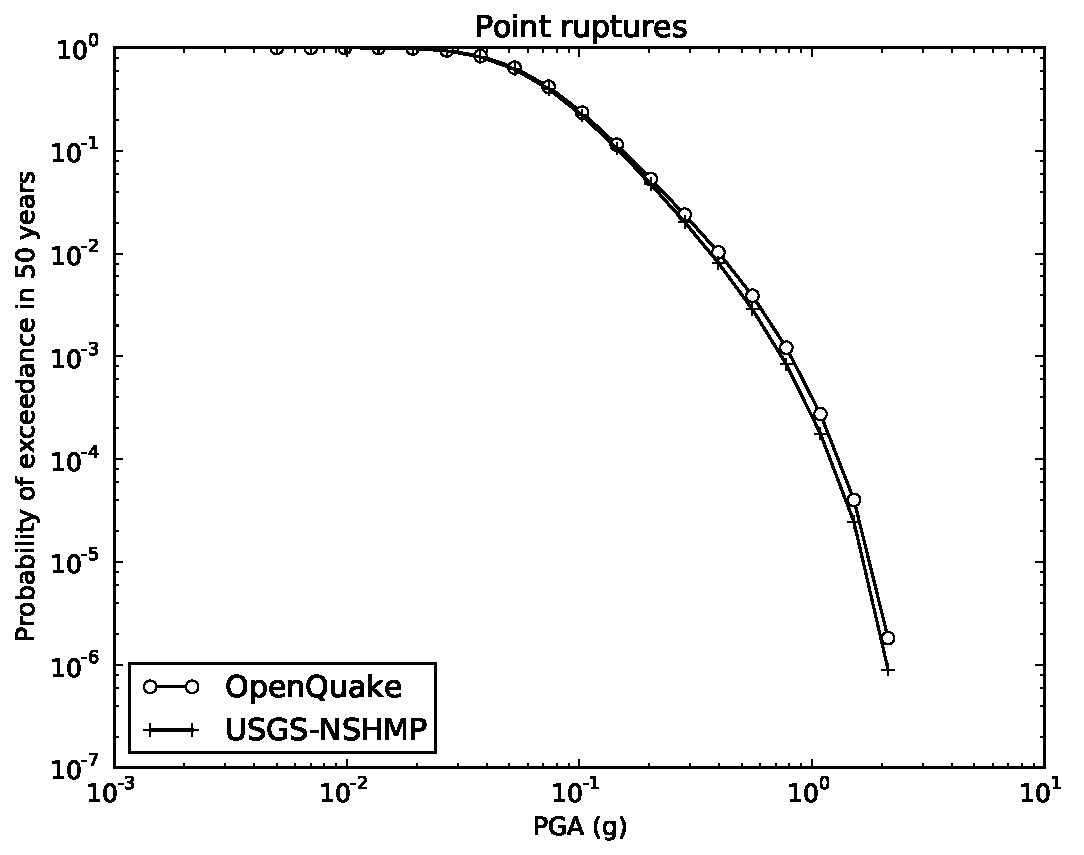
\includegraphics[width=10cm]{./qareport/pictures/-120pt7_36pt31_point.pdf}
\caption{Hazard curve comparison for site with coordinates -120.7E, 36.31N assuming \textit{point ruptures}}
\label{fig:cal_grid_curve_point}
\end{figure}

\begin{figure}
\centering
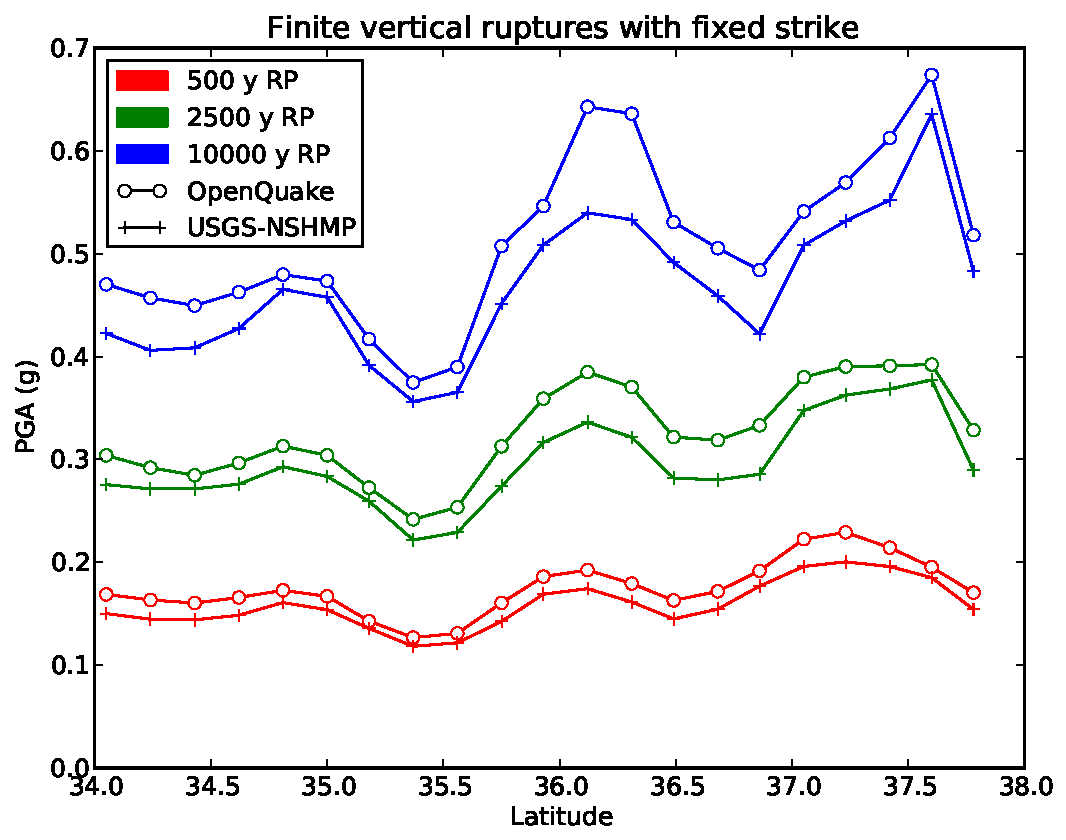
\includegraphics[width=10cm]{./qareport/pictures/gridded_seismicity_oq_nshmp_fixedstrikevertical.pdf}
\caption{Comparison of hazard map values for different return periods (RP) along the profile assuming finite vertical ruptures with fixed strike.}
\label{fig:cal_grid_map_finite}
\end{figure}

\begin{figure}
\centering
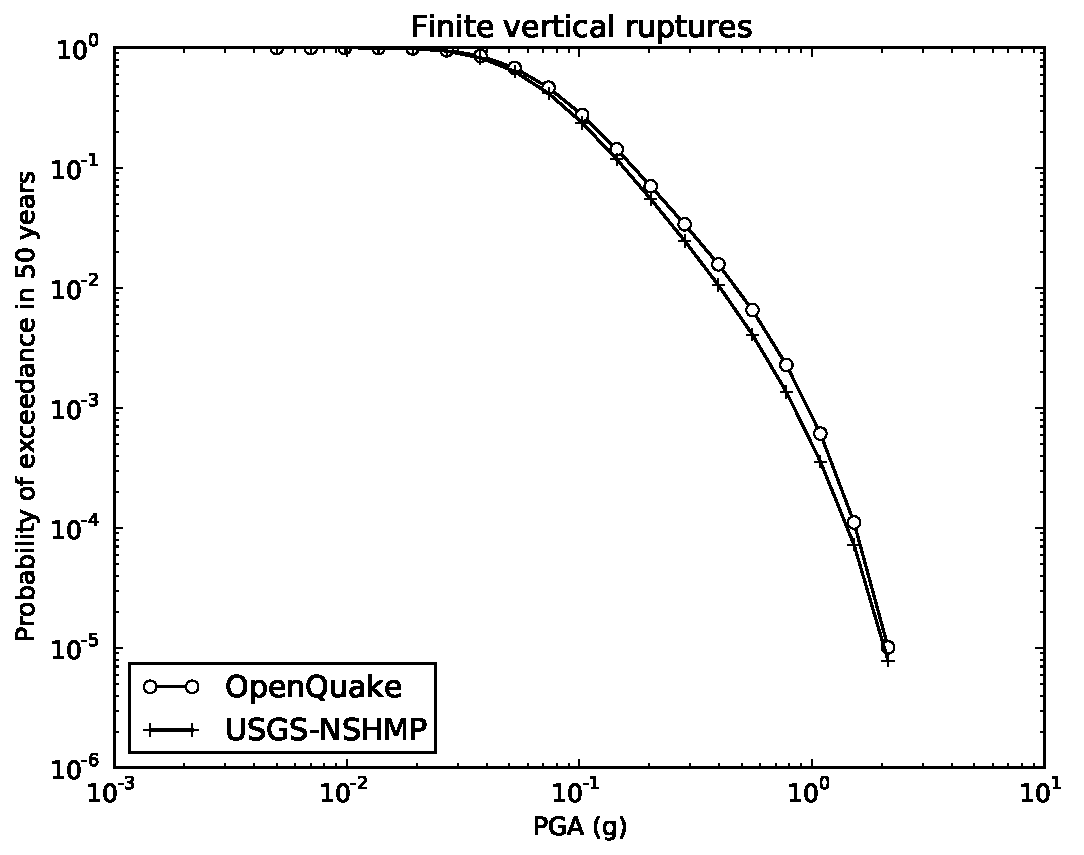
\includegraphics[width=10cm]{./qareport/pictures/-120pt7_36pt31_fixedstrikevertical.pdf}
\caption{Hazard curve comparison for site with coordinates -120.7E 36.31N assuming finite vertical ruptures with fixed strike.}
\label{fig:cal_grid_curve_finite}
\end{figure}

\subsection{Benchmarks for crustal faults}
As benchmarks for crustal faults, we considered two fault models for the State of California. One based on type-A faults (\cite{petersen2008}), which defines only characteristic fault sources (Figure \ref{fig:type_a_fault}) and one based on type-B faults (Figure \ref{fig:type_b_fault}), which contain mostly Gutenberg-Richter fault sources. Both source models are associated with the USGS-NSHMP computer program \textit{hazFXnga7c.f}.

% Type-A fault
\begin{figure}[htb]
\centering
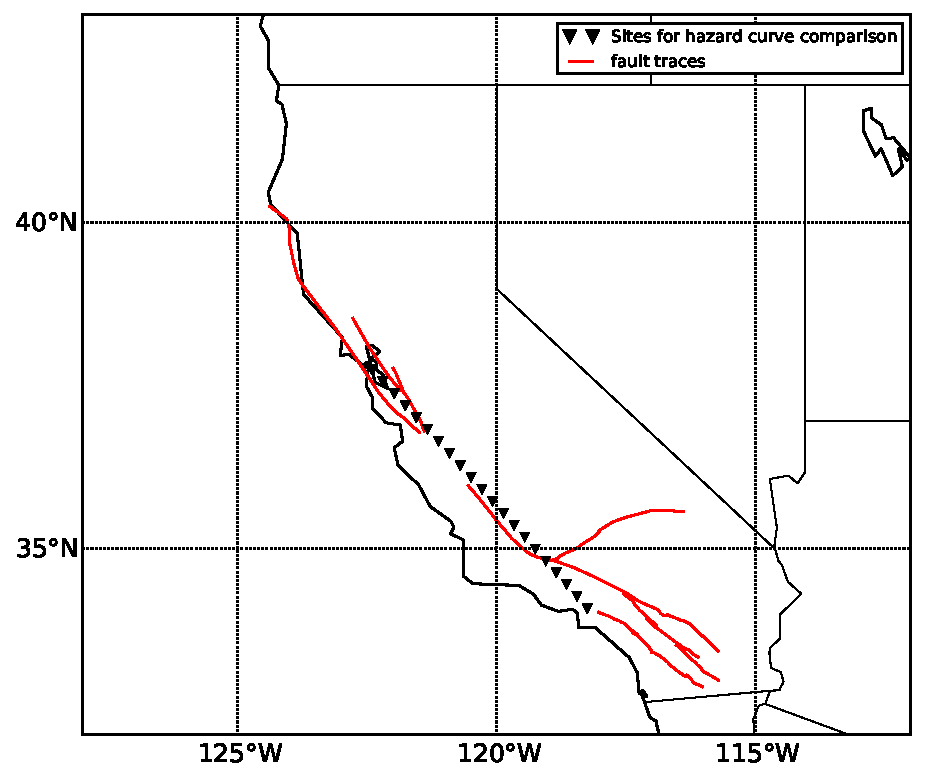
\includegraphics[width=10cm]{./qareport/pictures/aFault_aPriori_D2pt1.pdf}
\caption{Type-A fault model}
\label{fig:type_a_fault}
\end{figure}

% Type-B fault
\begin{figure}[htb]
\centering
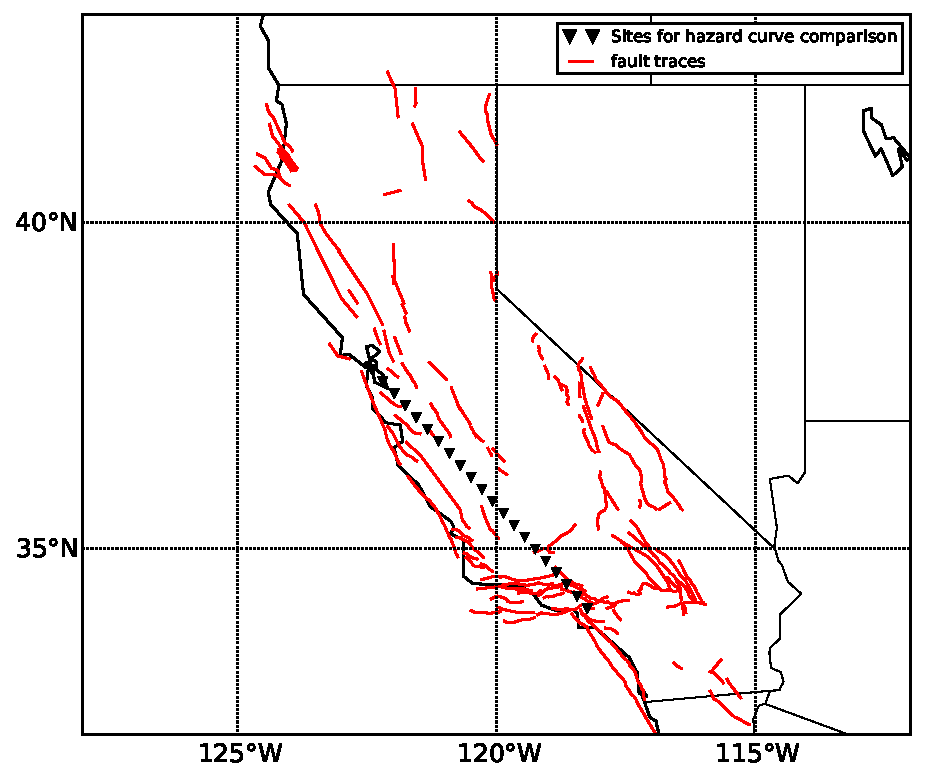
\includegraphics[width=10cm]{./qareport/pictures/bFault_stitched_D2pt1_GR0.pdf}
\caption{Type-B fault model}
\label{fig:type_b_fault}
\end{figure}

Characteristic faults are defined through a Normal (i.e. Gaussian) magnitude-frequency distribution. For each magnitude-bin, the entire fault surface is assumed to rupture. In a characteristic model no scaling relationship is required, and hence floating ruptures are not modeled. On the contrary, in a Gutenberg-Richter fault, ruptures are floated only along the fault strike and rupture extension is modeled in terms of a magnitude-length scaling relationship. The magnitude-length scaling is actually derived from the magnitude-area scaling relationship of \citet{hanks2002} and assuming a fixed width (equal to the fault width).

We compare hazard curves for the same set of locations as for the distributed seismicity model. Results of the comparison are given in Figures \ref{fig:type_a_map} and \ref{fig:type_a_curve} for the type-A fault model, and \ref{fig:type_b_map}, and \ref{fig:type_b_curve} for the type-B fault model. For the type-A fault model, the agreement between the USGS-NSHMP and OpenQuake-engine solutions is very good. When considering instead the results from the type-B fault model some discrepancies are visibile, especially for return periods longer than 500 years, altough the level of agreement is still acceptable. The lack of a complete agreement in the type-B fault model solutions may indicate the effect of differences in the rupture floating algorithm between the two software. In the OpenQuake-engine the magnitude-area scaling relationship of \citet{wells1994} is used and rupture floating occurs both along strike and dip. Indeed, the very good agreement in the case of the type-A fault model (which does not consider any rupture floating) confirms that the modeling of rupture extension and location on a fault surface plays an important role in the hazard calculation procedure.

\begin{figure}
\centering
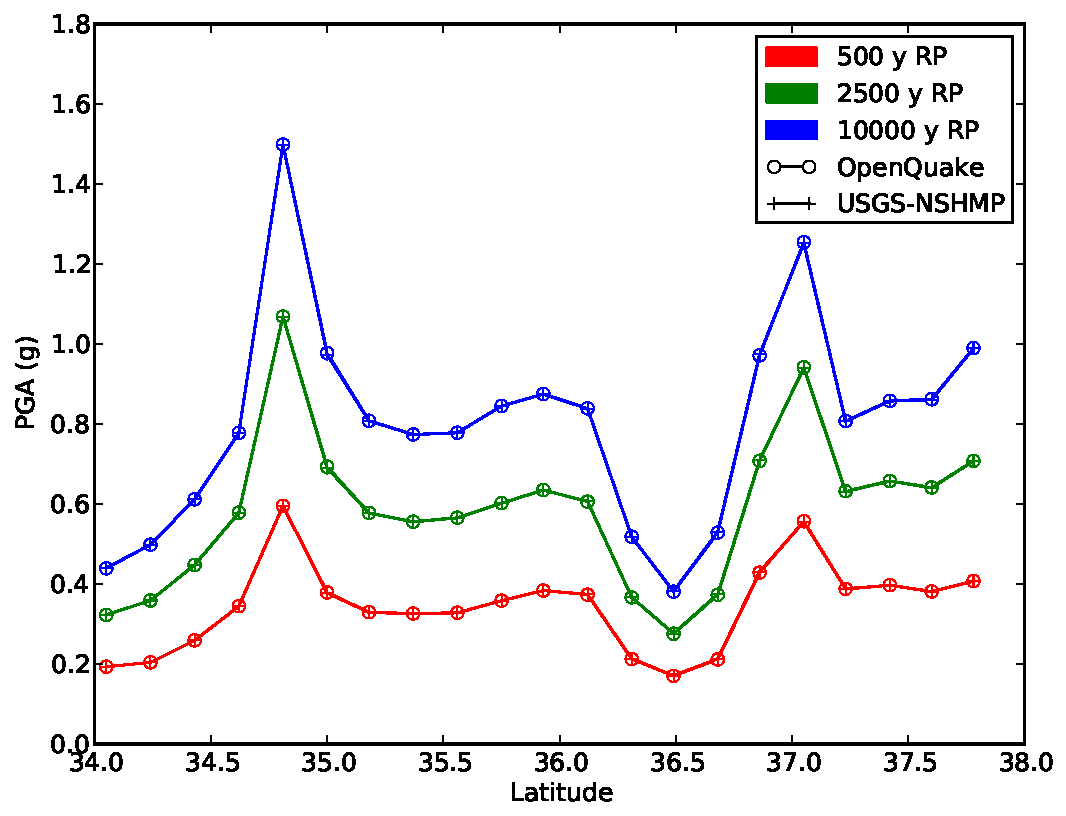
\includegraphics[width=10cm]{./qareport/pictures/oq_nshmp_aFault.pdf}
\caption{Hazard map comparison for Type-A fault model.}
\label{fig:type_a_map}
\end{figure}
\begin{figure}
\centering
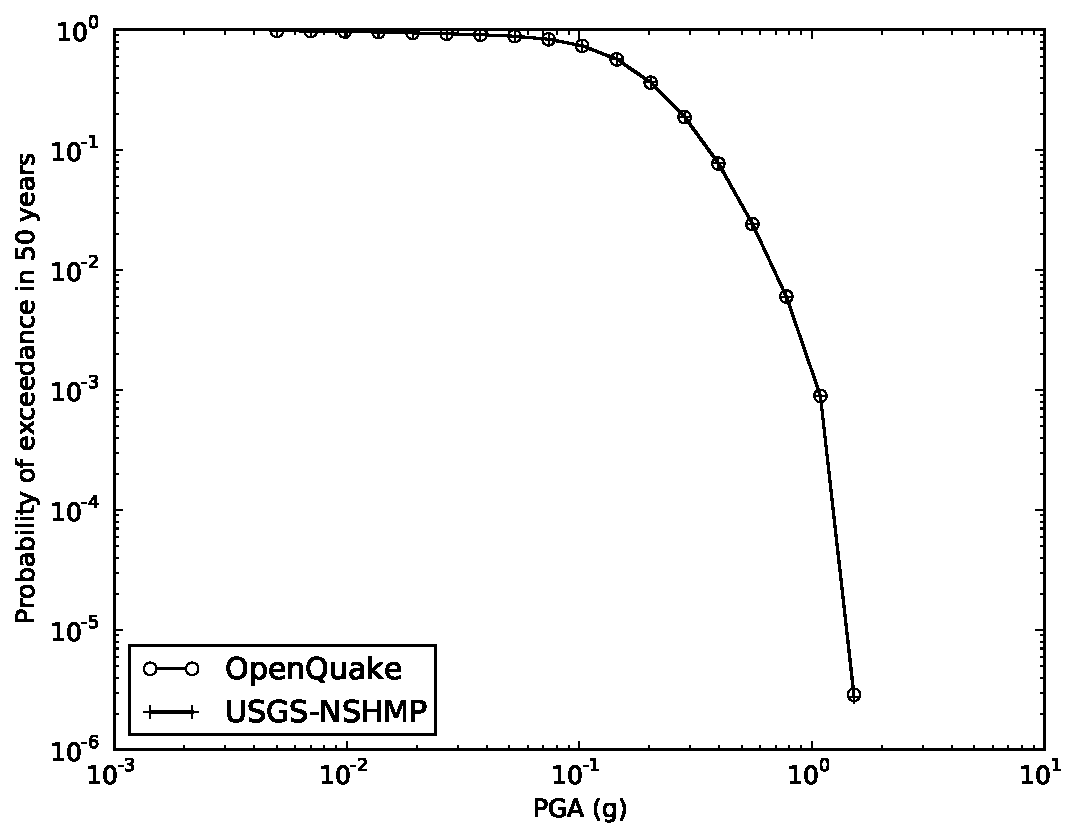
\includegraphics[width=10cm]{./qareport/pictures/-120pt49_36pt12_aFault.pdf}
\caption{Hazard curve comparison for site with coordinates -120.49E 36.12N using Type-A fault model}
\label{fig:type_a_curve}
\end{figure}

\begin{figure}
\centering
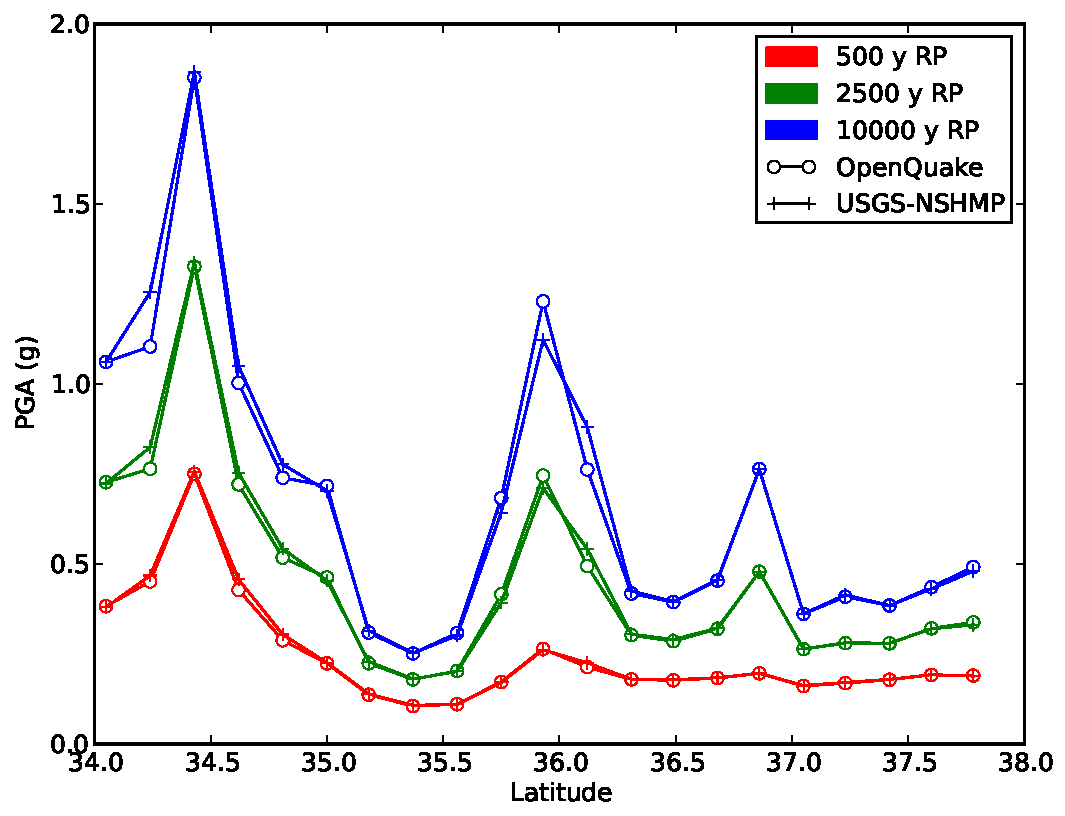
\includegraphics[width=10cm]{./qareport/pictures/oq_nshmp_bFault_ar1.pdf}
\caption{Hazard map comparison for Type-B fault model}
\label{fig:type_b_map}
\end{figure}
\begin{figure}
\centering
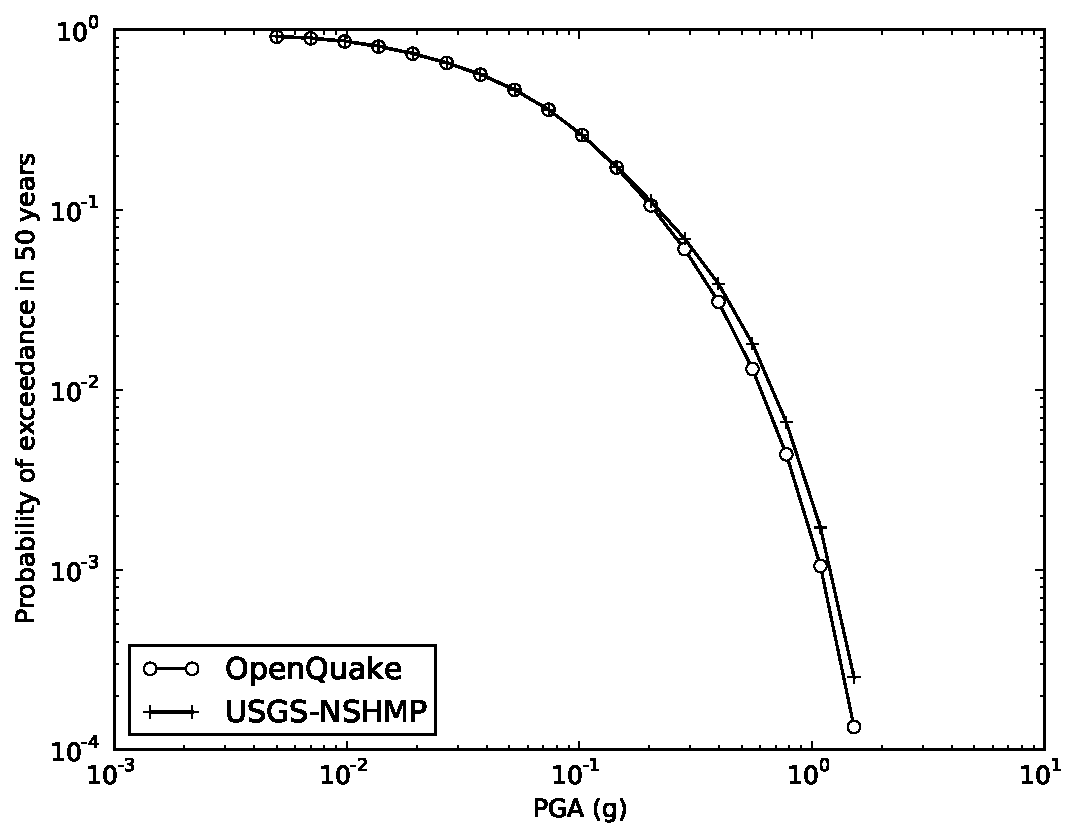
\includegraphics[width=10cm]{./qareport/pictures/-120pt49_36pt12_bFault_ar1.pdf}
\caption{Hazard curve comparison for site with coordinates -120.49E 36.12N using Type-B fault model}
\label{fig:type_b_curve}
\end{figure}

\subsection{Benchmarks for subduction faults}
The 2008 U.S. national seismic hazard model (\cite{petersen2008}) defines fault sources with complex geometries to model large subdaction interface faults in the Cascadia region. We thus selected a fault model for the Cascadia region as a benchmark for the modeling of complex fault sources.

Similarly to what done for crustal sources, we considered a characteristic model (where earthquakes always rupture the entire fault surface) and an unsegmented model where ruptures (whose extension is constrained by a scaling relationship) are allowed to move along the entire fault surface. The characteristic model defines a single event of magnitude ($M_{w}=9.2$) which breaks a complex fault surface depicted in Figure \ref{fig:cascadia_geo}. The unsegmented model defines the same fault geometry, however earthquake ruptures are generated from minimum magnitude 8.3 to maximum magnitude 8.7. Ruptures are floated only along the strike direction and rupture length is obtained from a magnitude-length scaling relationship specific for the Cascadia region. Both source models are associated with the USGS-NSHMP computer program \textit{hazSUBXnga.f}. To perfom a more fair comparison againt the OpenQuake-engine we modified the \textit{hazSUBXnga.f} code so that rupture length is computed from the \citet{wells1994} magnitude-area scaling relationship and assuming a rupture aspect ratio equal to 1.

Hazard curves are compared along two profiles, aligned along the E-W and N-S directions. When considering the characteristic model, the agreement between the solutions provided by the two software is very good (Figures \ref{fig:cascadia_char_ew}, \ref{fig:cascadia_char_ns}). On the contrary, when considering the unsegmented model (Figures \ref{fig:cascadia_float_ew} and \ref{fig:cascadia_float_ns}) large discrepancies are evident especially along the N-S profile. The large discrepancies can be understood again in terms of the differences between the rupture floating algorithm in the two software. In particular, the USGS-NSHMP code define rupture extension along length only and assume each rupture to extend along dip until the fault bottom edge. In the OQ-engine instead, rupture extension and shape is determined by a magnitude-area scaling relationship and rupture aspect-ratio, and each rupture can be moved both along strike and along dip. The bulge in the hazard map profiles as visible in Figure \ref{fig:cascadia_float_ns} can be explained in terms of a large number of ruptures modelled by the OQ-engine in the inner part of the fault surface. In the USGS-NSHMP approach, the number of ruptures along the fault surface is constant, as also demonstrated by the constant hazard values along the N-S profile.
\begin{figure}
\centering
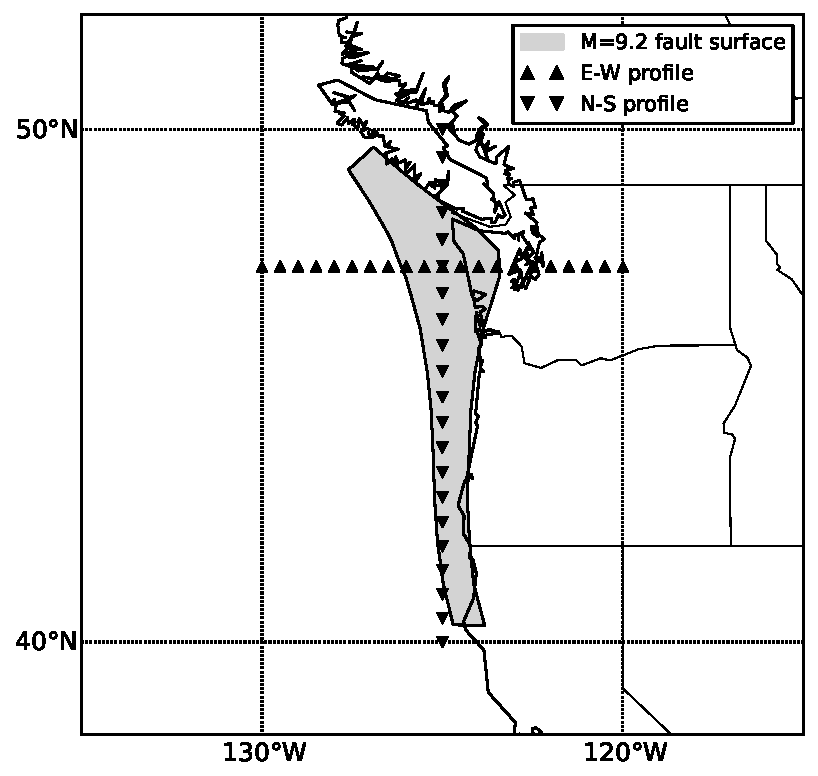
\includegraphics[width=10cm]{./qareport/pictures/cascadia_char.pdf}
\caption{Cascadia characteristic fault model ($M_{w}$=9.2)}
\label{fig:cascadia_geo}
\end{figure}

\begin{figure}
\centering
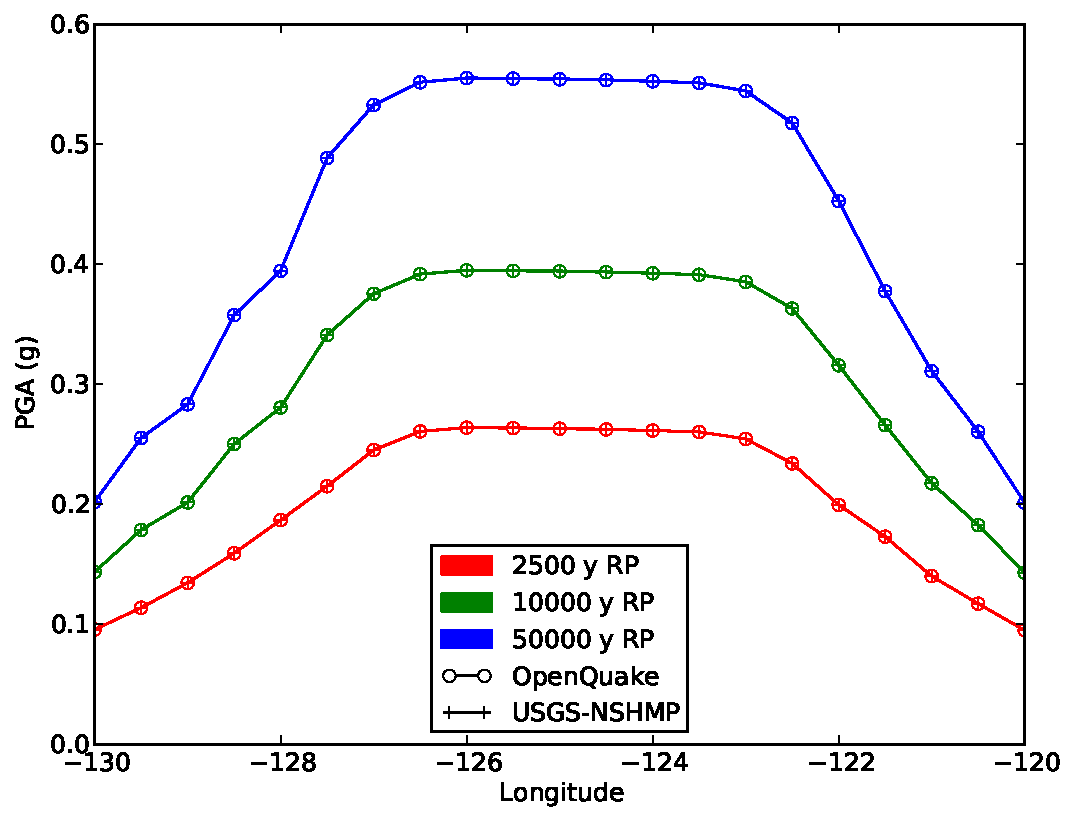
\includegraphics[width=10cm]{./qareport/pictures/cascadia_char_oq_nshmp_ew.pdf}
\caption{Hazard map comparison along EW profile for Cascadia characteristic model}
\label{fig:cascadia_char_ew}
\end{figure}
\begin{figure}
\centering
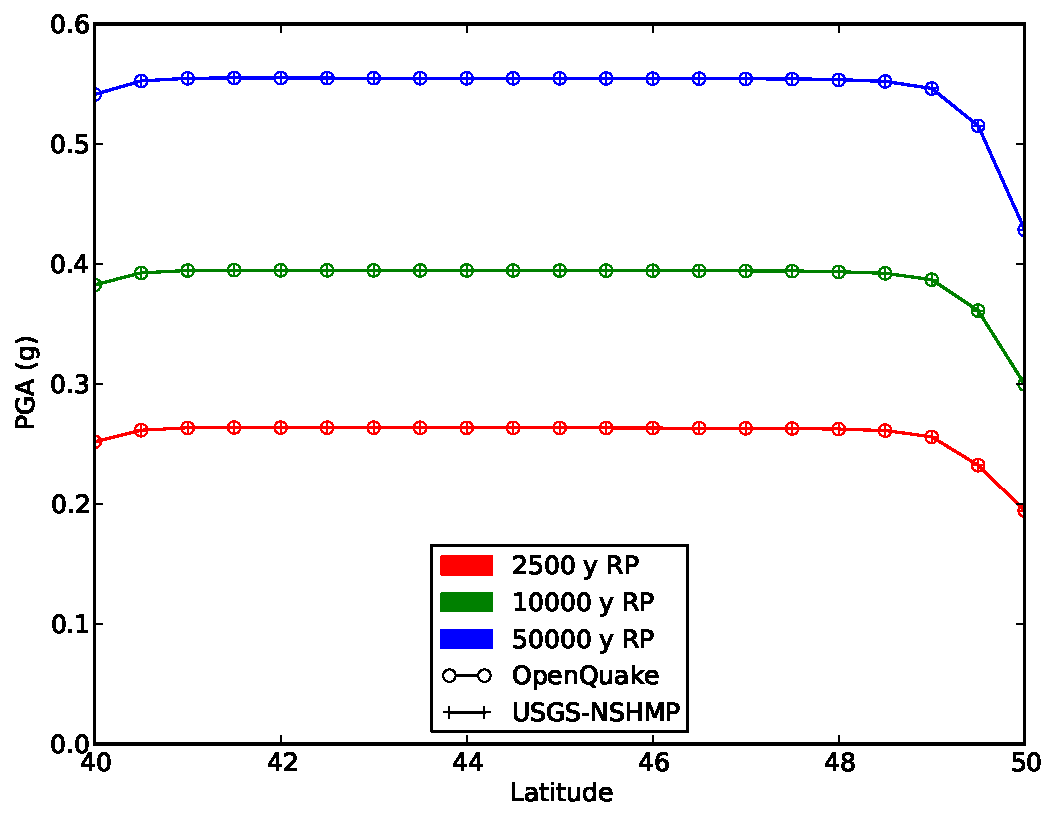
\includegraphics[width=10cm]{./qareport/pictures/cascadia_char_oq_nshmp_ns.pdf}
\caption{Hazard map comparison along NS profile for Cascadia characteristic model}
\label{fig:cascadia_char_ns}
\end{figure}

\begin{figure}
\centering
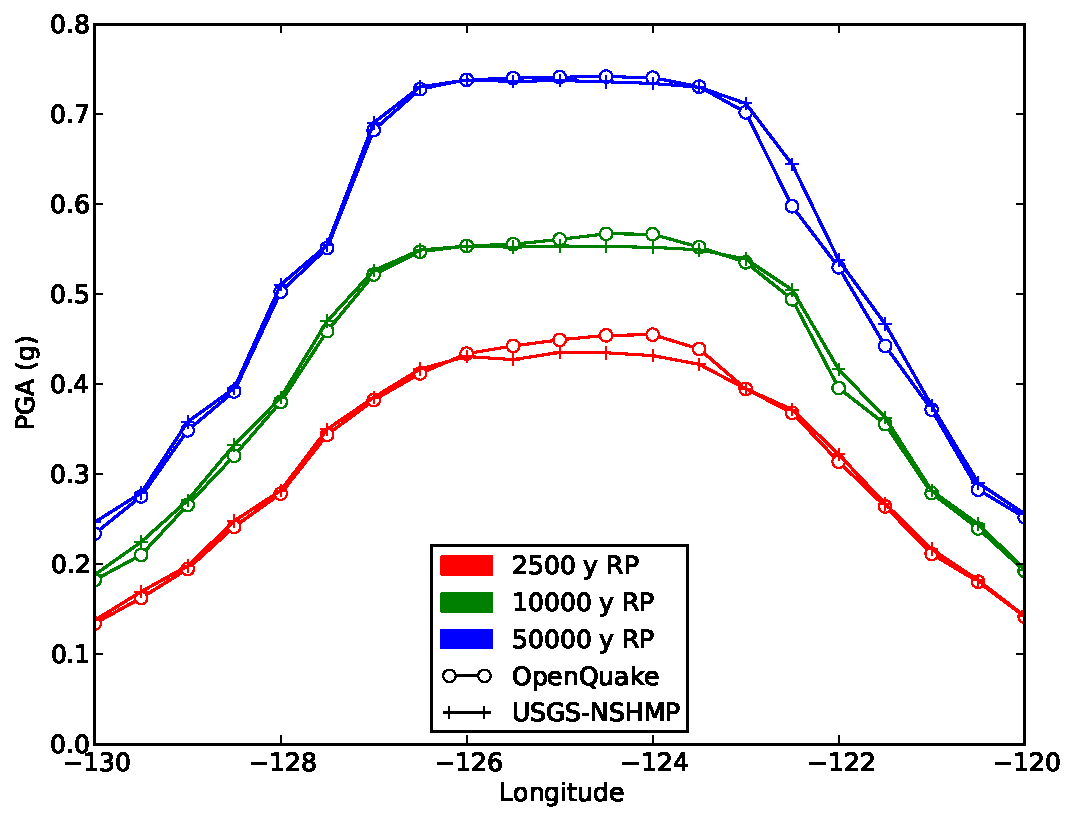
\includegraphics[width=10cm]{./qareport/pictures/cascadia_float_oq_nshmp_ew.pdf}
\caption{Hazard map comparison along EW profile for Cascadia unsegmented model}
\label{fig:cascadia_float_ew}
\end{figure}
\begin{figure}
\centering
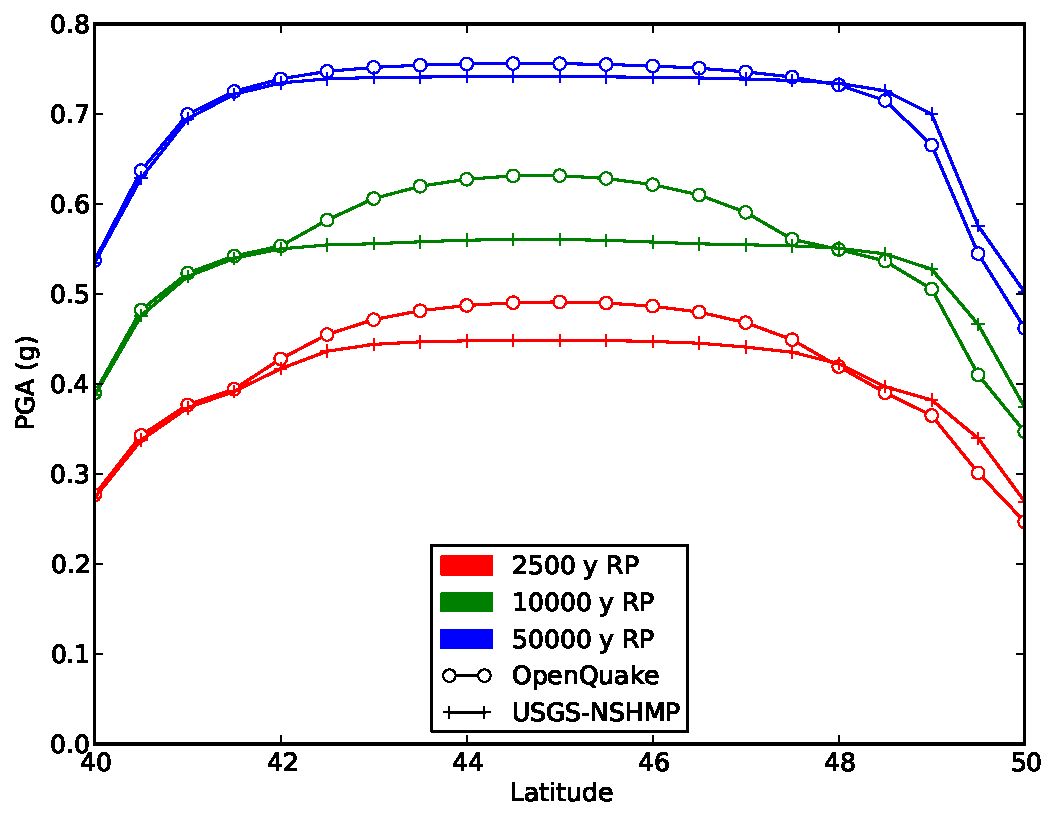
\includegraphics[width=10cm]{./qareport/pictures/cascadia_float_oq_nshmp_ns.pdf}
\caption{Hazard map comparison along NS profile for Cascadia unsegmented model}
\label{fig:cascadia_float_ns}
\end{figure}
